\documentclass[11pt,letterpaper,boxed]{hmcpset}
\usepackage{fullpage}
\setlength{\parskip}{6pt}
\setlength{\parindent}{0pt}
\usepackage[margin=1in]{geometry}
\usepackage{graphicx}
\usepackage{enumerate}
\usepackage{marvosym}
\usepackage{amssymb}
\usepackage{wasysym}
\usepackage{gensymb}
\usepackage{mathrsfs}
\usepackage{scrextend}
\usepackage{mathtools}
\usepackage{pgfplots}
\usepackage{xspace}
\usepackage{esvect}

\name{Name $\rule{4cm}{0.15mm}$}
\class{Physics 51M Section $\rule{.5cm}{0.15mm}$ Box \# $\rule{1cm}{0.15mm}$}
\assignment{Problem Set 5}
\duedate{14 October 2019}

\begin{document}
	
	%\begin{center}
	\noindent\textbf{Collaborators:} 
	%\end{center} 
	
	%\problemlist{}
	
	\begin{problem}[Problem 1]
		
		\begin{enumerate}
			\item [(a)] Calculate a line integral of a vector function
			$\vec{G}(x,y,z) = z^2 \hat x + x^2 \hat y - y^2 \hat z$ over a path $C_3$ in the $(x-y)$ plane, as shown in the figure.
			\item [(b)] Now repeat the calculation over the piecewise path $C_1+C_2$.
			\item [(c)] A vector field is called conservative if its line
			integral is path independent between any two endpoints.  Based on your results above, is $\vec{G}$ a conservative vector field?
		\end{enumerate}
	
		\begin{center}
			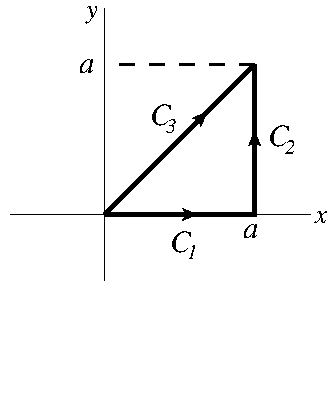
\includegraphics[width=4cm]{hw5-fig}
		\end{center}
		
		
	\end{problem}
	
	\begin{solution}
		\vfill
	\end{solution}
	\newpage
	
	
	\begin{problem}[Problem 2]
		Calculate the work done by the force $\vec F = -y
		\hat x + x \hat y$ along the closed path defined by the parametric trajectory 
		
		\[\vec r (t) = a \cos{\left(\frac{t}{t_0}\right)} \hat x + a
		\sin{\left(\frac{t}{t_0}\right)} \hat y + a \cos{\left(\frac{2 t}{t_0}\right)} \hat z\] 
		
		where $a$ and $t_0$ are constants with appropriate units.   Is $\vec{F}$ a conservative vector field?  
		\\
		\\{\em Hint:} Start by justifying that $t=0$ and $t=2 \pi t_0$ give valid starting and ending integration points.  		
		
	\end{problem}
	
	\begin{solution}
		\vfill
	\end{solution}
	\newpage
	
	
	\begin{problem}[Problem 3*]
		Suppose an electric field is given by $\vec{E} = k
		\frac{\hat r}{r}$ in spherical coordinates, where $k$ is a
		constant.
		
		\begin{enumerate}
			\item [(a)] Find the volume charge density $\rho$ everywhere in space.
			\item [(b)] Using Gauss’s Law, find the total charge contained
			in a sphere of radius $R$, centered at the origin (at $r = 0$).
			\item [(c)] Repeat part (b), but this time find the total
			charge by direct integration of $\rho$ over the volume of the sphere. Do you get the same result?
		\end{enumerate}
			
	\end{problem}
	
	\begin{solution}
		\vfill
	\end{solution}
	\newpage
	
	
	\begin{problem}[HRK E28.2]
		Derive an expression for the work required by an external agent to put the four charges together as indicated in Fig 28-28. Each side of the square has length $a$.
		
		\begin{center}
			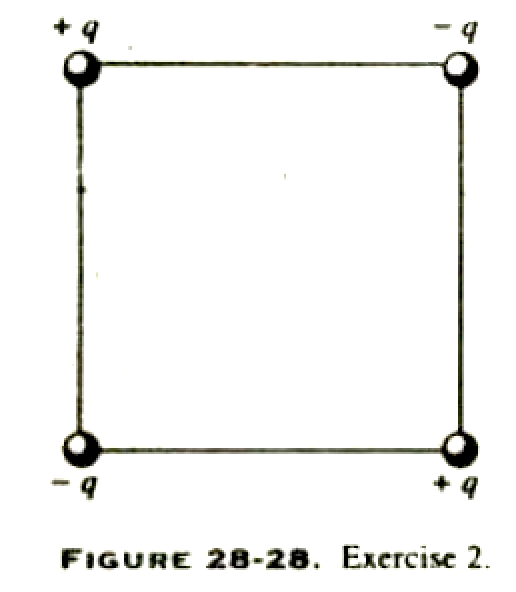
\includegraphics[scale=0.4]{28-28.png}
		\end{center}
		
	
		
	\end{problem}
	
	\begin{solution}
		\vfill
	\end{solution}
	\newpage
	
	
	\begin{problem}[HRK P28.6]
		A particle of mass $m$, charge $q>0$, and initial kinetic energy $K$ is projected (from an infinite separation) toward a heavy nucleus of charge $Q$, assumed to have a fixed position in our reference frame.
		
		\begin{enumerate}
			\item [(a)] If the aim is ``perfect'', how close to the center of the nucleus is the particle when it comes instantaneously to rest?
			\item [(b)] With a particular imperfect aim, the particle's closest approach to the nucleus is twice the distance determined in part $(a)$. Determine the speed of the particle at this closest distance of approach. Assume that the particle does not reach the surface of the nucleus.
		\end{enumerate}

		
	\end{problem}
	
	\begin{solution}
		\vfill
	\end{solution}
	\newpage
	
	
	\begin{problem}[HRK P28.10]
		A total amount of positive charge $Q$ is spread onto a nonconducting, flat, circular annulus of inner radius $a$ and outer radius $b$. This charge is distributed so that the charge density (charge per unit area) is given by $\sigma = k/r^3$, where $r$ is the distance from the center of the annulus to any point on it. Show that (with $V = 0$ at infinity) the potential at the center of the annulus is given by
		
		\[V = \frac{Q}{8\pi \epsilon_0}\left(\frac{a+b}{ab}\right)\]
		
	\end{problem}
	
	\begin{solution}
		\vfill
	\end{solution}
	
	
\end{document}